\section{Problem 3}

\subsection{Fitting result without regularization}

I tuned the $\alpha$ from [0.001, 0.01, 0.1] and $n_{epoch}$ from [100000, 500000, 1000000]. But actually, with the help of early stopping criterion, we only needs the largest number of epochs. So I only show the result for $n_{epoch} = 1000000$, with varying $\alpha$. Different learning rates do not make the results that different. The lowest error rate is 16.1\%.

\begin{figure}[H]
\centering
  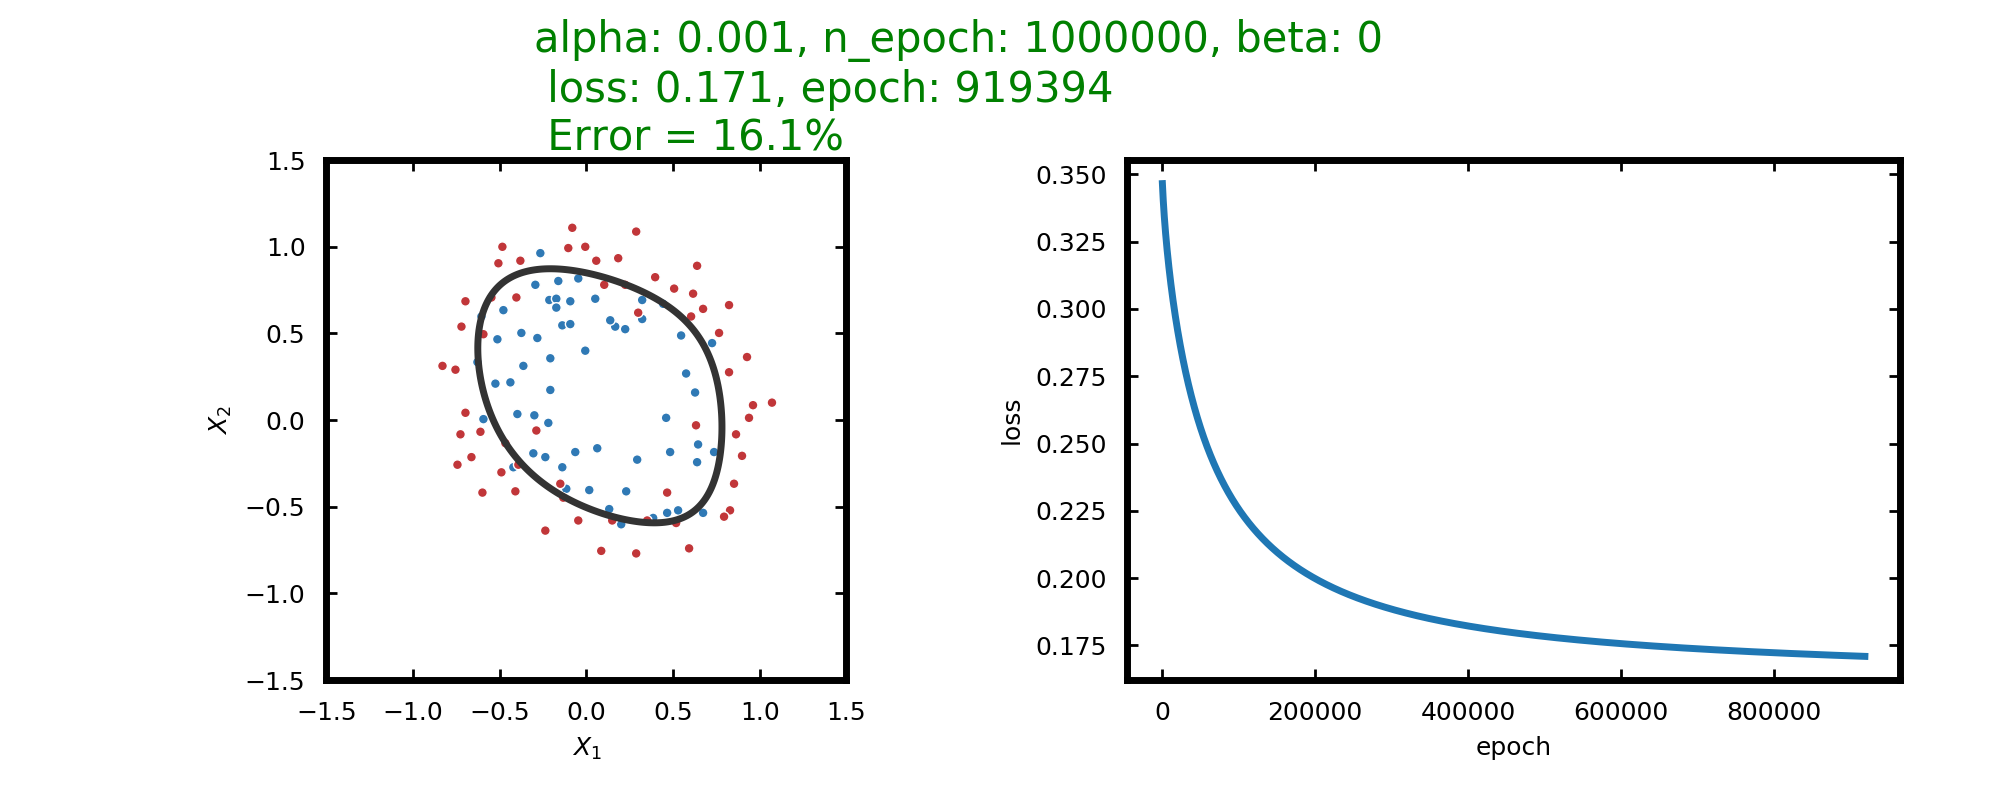
\includegraphics[width=0.85\textwidth]{fig/prob3/alpha_0_001_n_epoch1000000_beta_0.png}
\centering 
\caption{\protect $\alpha = 0.001$, $epoch = 1000000$}
\label{fig:15th}
\end{figure}

\begin{figure}[H]
\centering
  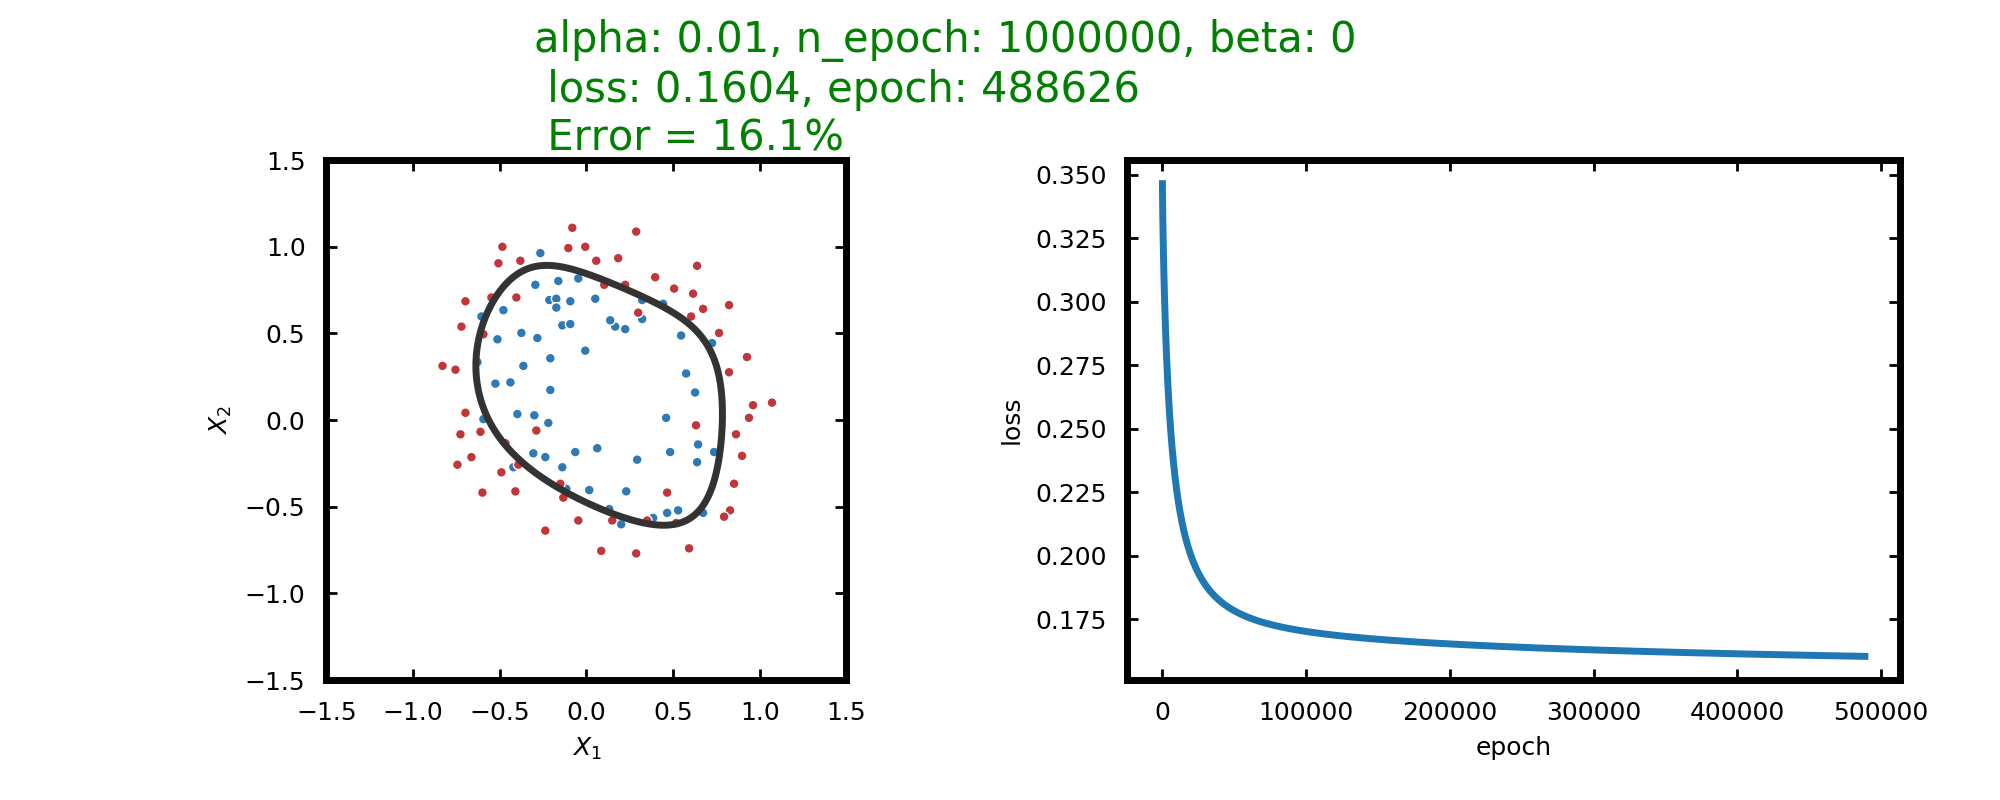
\includegraphics[width=0.85\textwidth]{fig/prob3/alpha_0_01_n_epoch1000000_beta_0.png}
\centering 
\caption{\protect $\alpha = 0.01$, $epoch = 1000000$}
\label{fig:15th}
\end{figure}

\begin{figure}[H]
\centering
  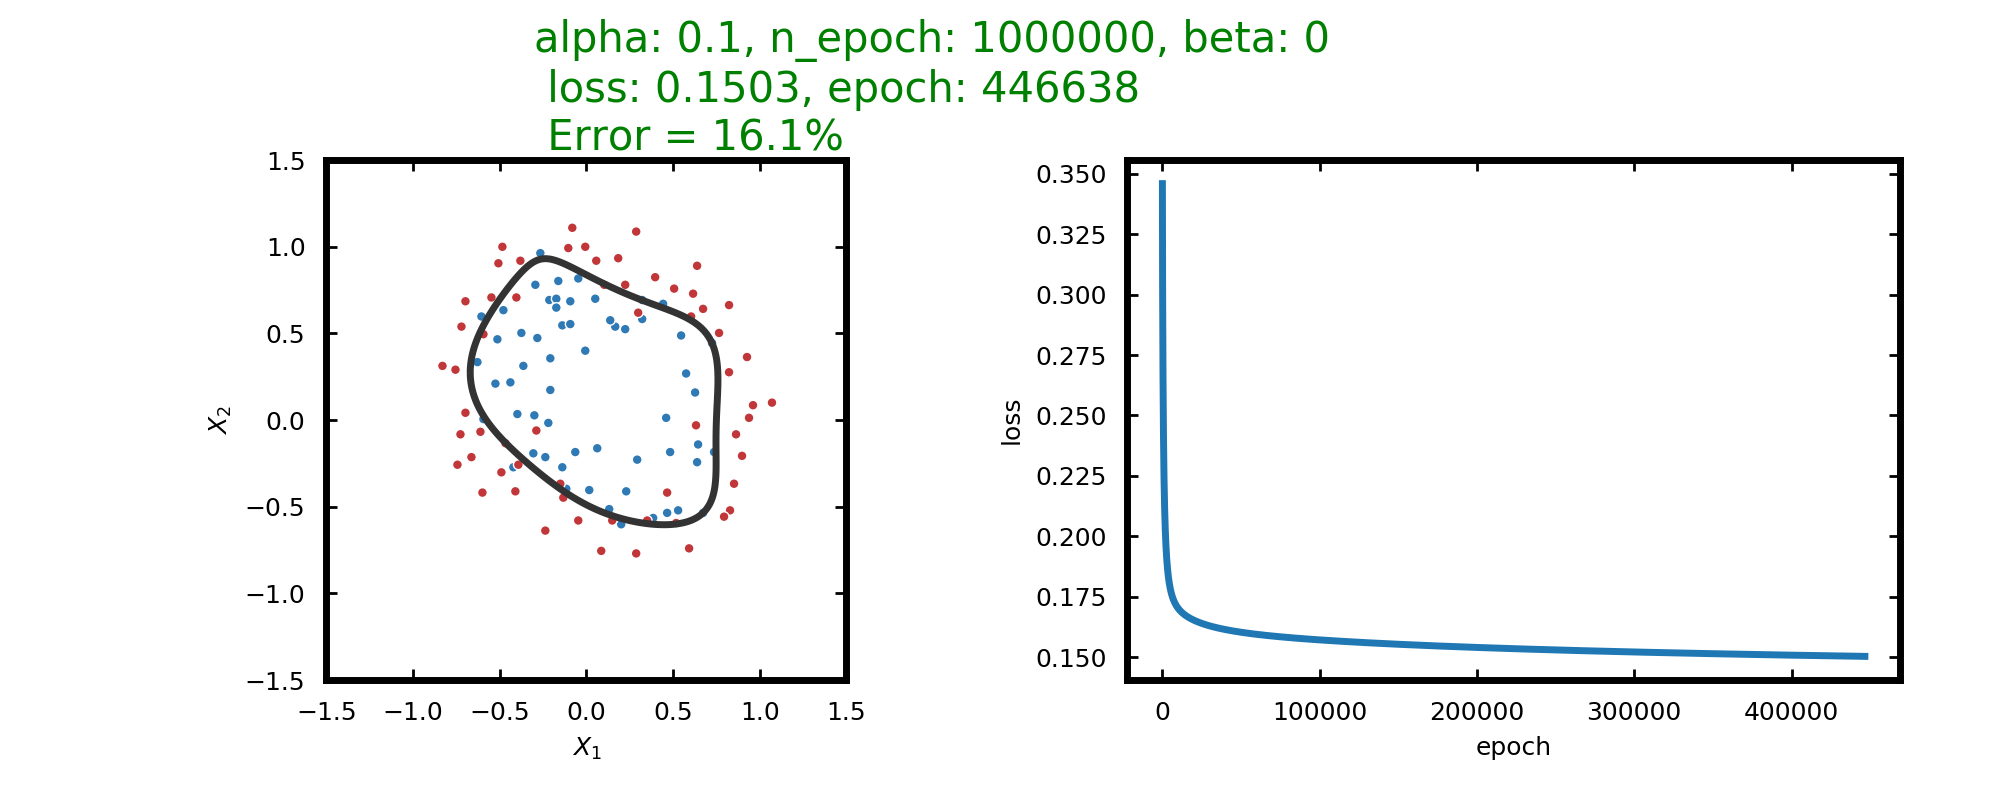
\includegraphics[width=0.85\textwidth]{fig/prob3/alpha_0_1_n_epoch1000000_beta_0.png}
\centering 
\caption{\protect $\alpha = 0.1$, $epoch = 1000000$}
\label{fig:15th}
\end{figure}

\subsection{Tuning the regularization}

I further tune the $\beta$ to change the regularization strength. With some proper strength of regularization (when $\beta \leq 0.1 $), the classification accuracy stays the same. When larger regularization is added, the accuracy starts to decrease. With increasing regularization, the decision boundary tends to be more smooth. 

Regularizing model will make the model more general and prevent it from overfitting.

The results is as below.

\begin{table}[htb]
\centering
\caption{Loss for different regularization}
\begin{tabular}{|l|l|}
\hline
$\beta$ & error rate \\ \hline
0. & 16.1\% \\ \hline
0.1 & 16.1\% \\ \hline
1 &  17.8\% \\ \hline
10 & 27.97\% \\ \hline
100 & 49.15\% \\ \hline
\hline
\end{tabular}
\label{tab:alpha}
\end{table}

\begin{figure}[H]
\centering
  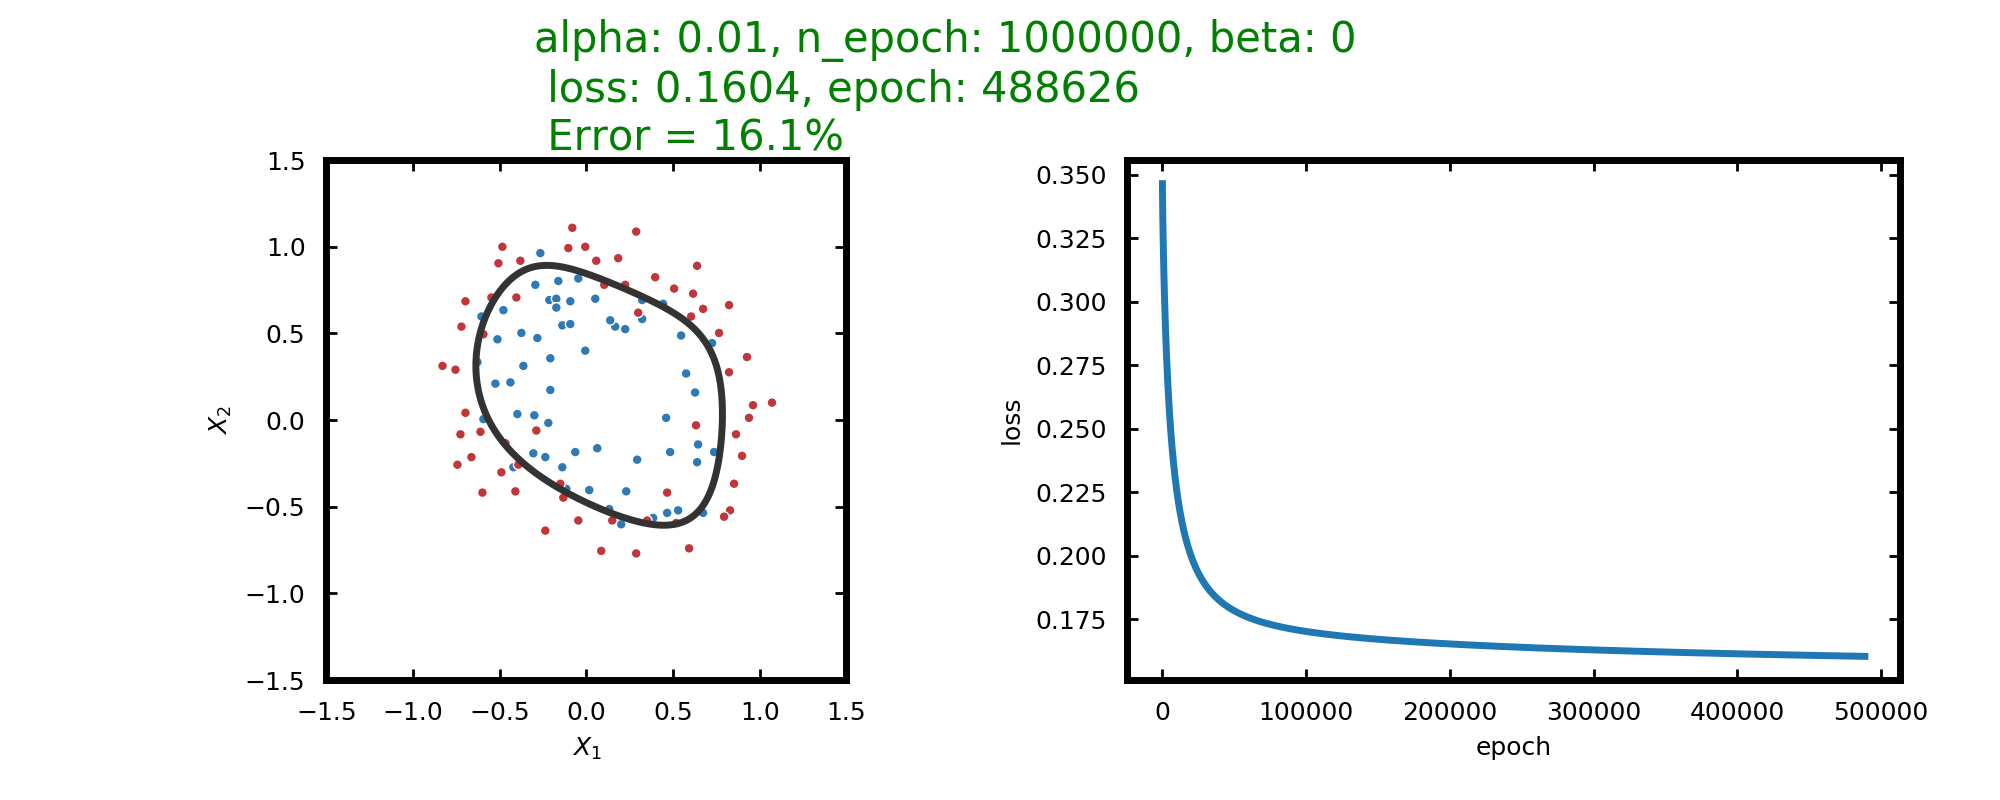
\includegraphics[width=0.85\textwidth]{fig/prob3/alpha_0_01_n_epoch1000000_beta_0.png}
\centering 
\caption{\protect No regularization}
\label{fig:15th}
\end{figure}

\begin{figure}[H]
\centering
  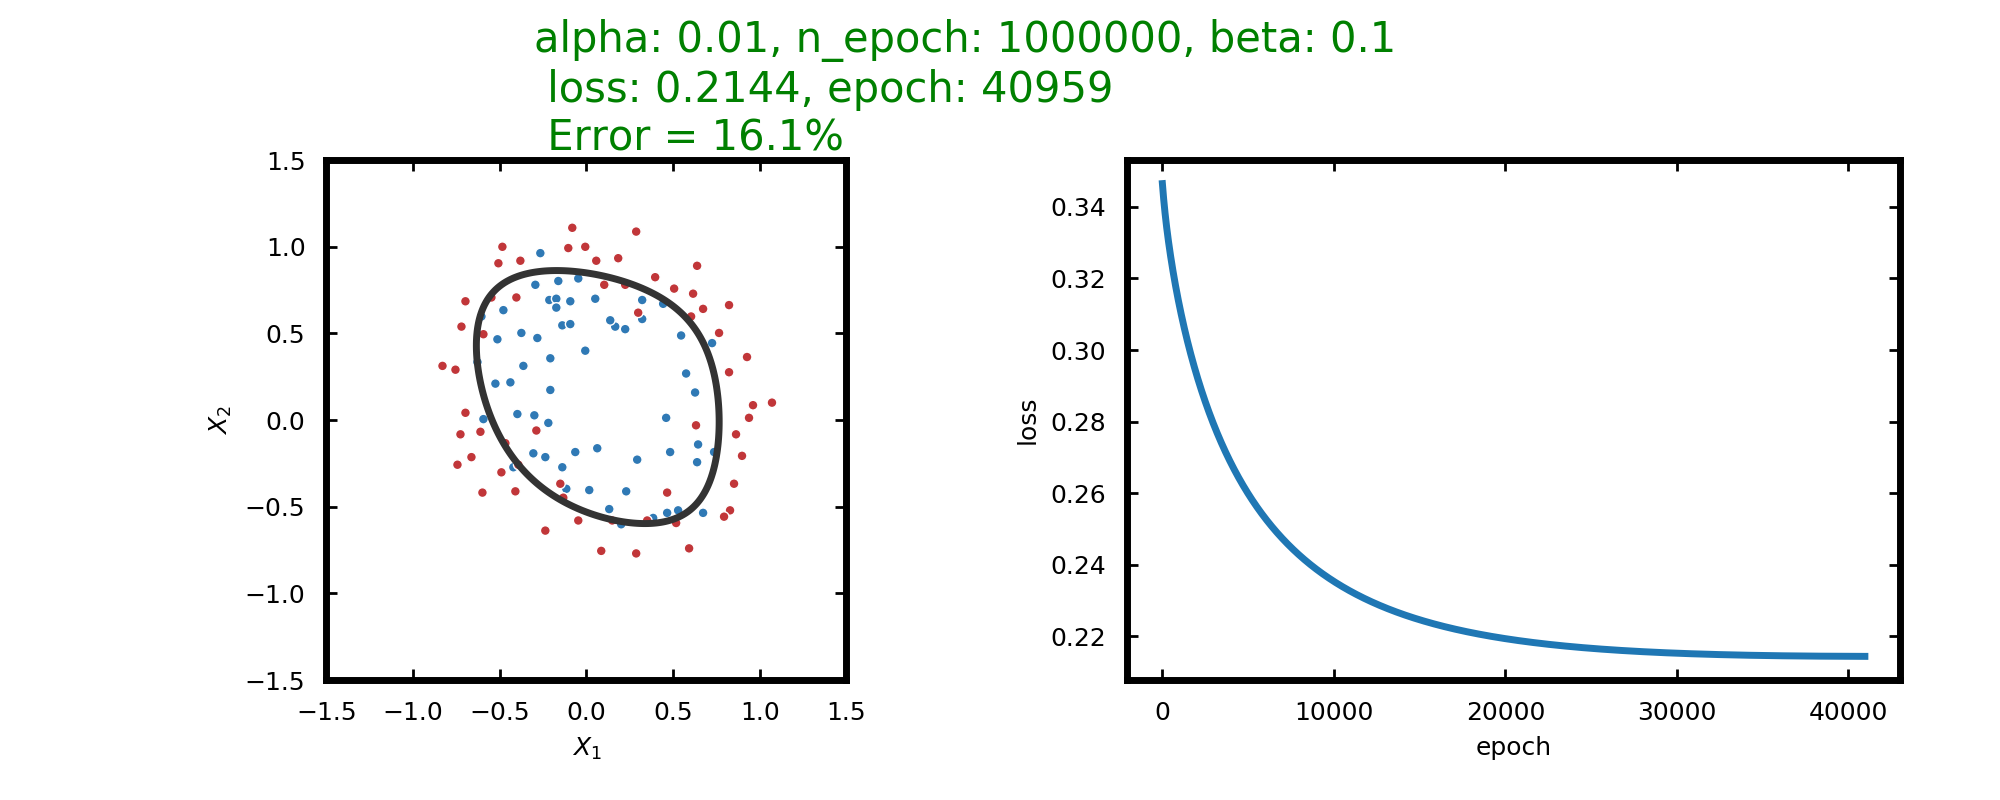
\includegraphics[width=0.85\textwidth]{fig/prob3/alpha_0_01_n_epoch1000000_beta_0_1.png}
\centering 
\caption{\protect $\beta = 0.1$}
\label{fig:15th}
\end{figure}

\begin{figure}[H]
\centering
  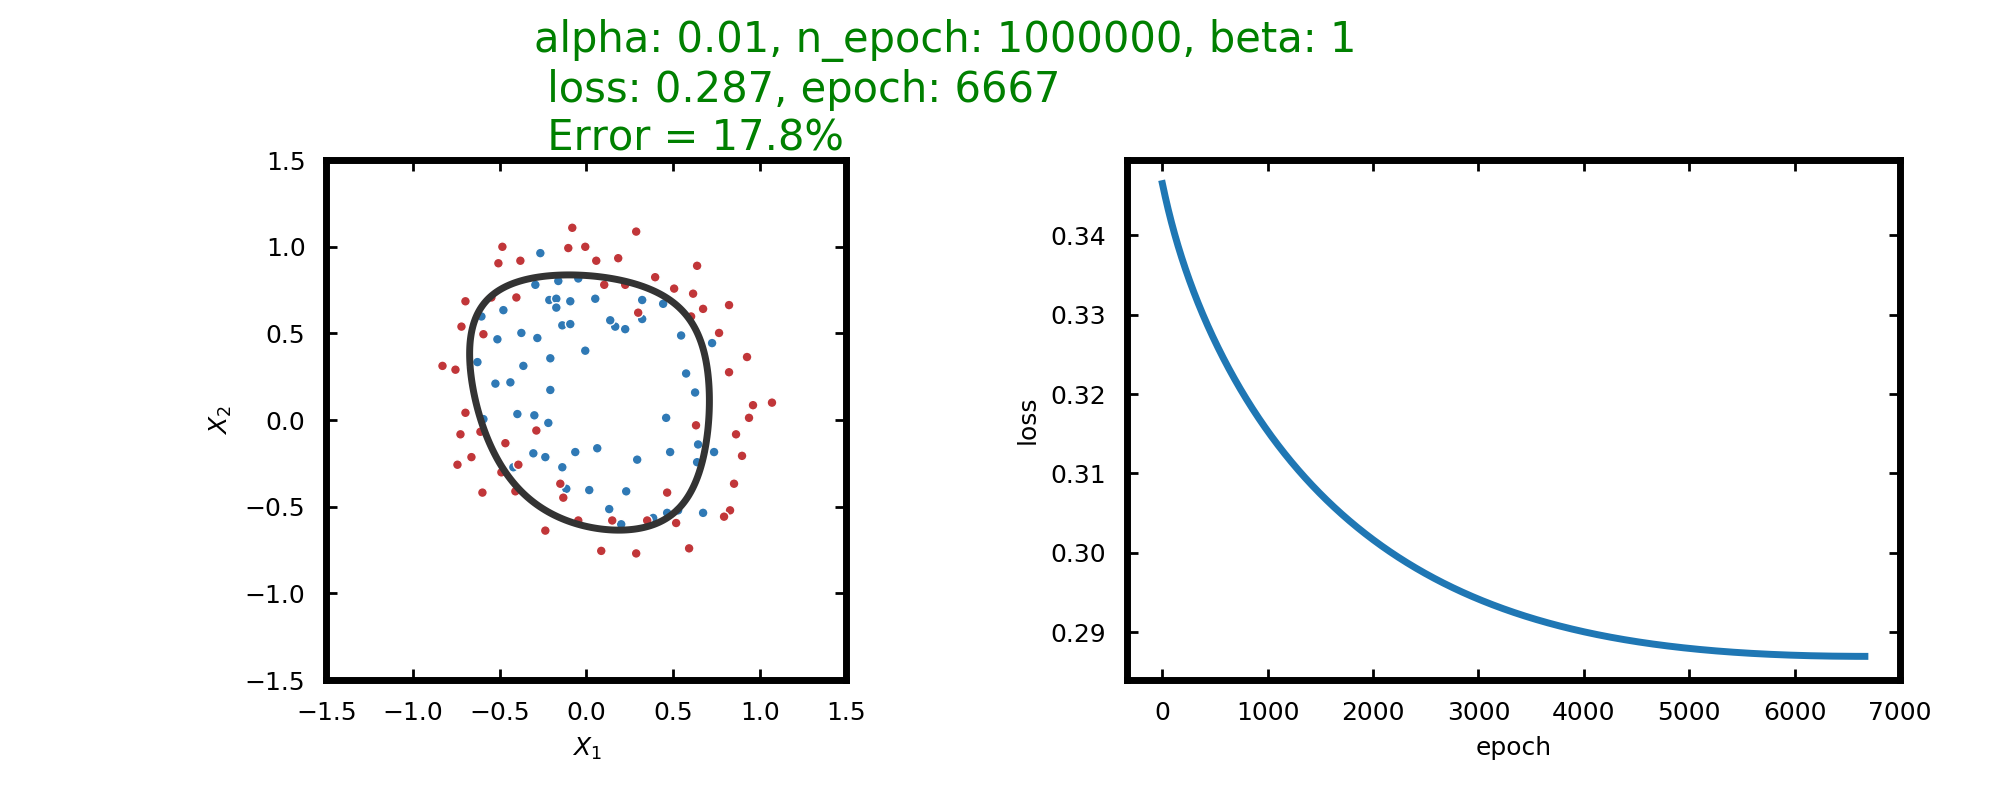
\includegraphics[width=0.85\textwidth]{fig/prob3/alpha_0_01_n_epoch1000000_beta_1.png}
\centering 
\caption{\protect $\beta = 1$}
\label{fig:15th}
\end{figure}

\begin{figure}[H]
\centering
  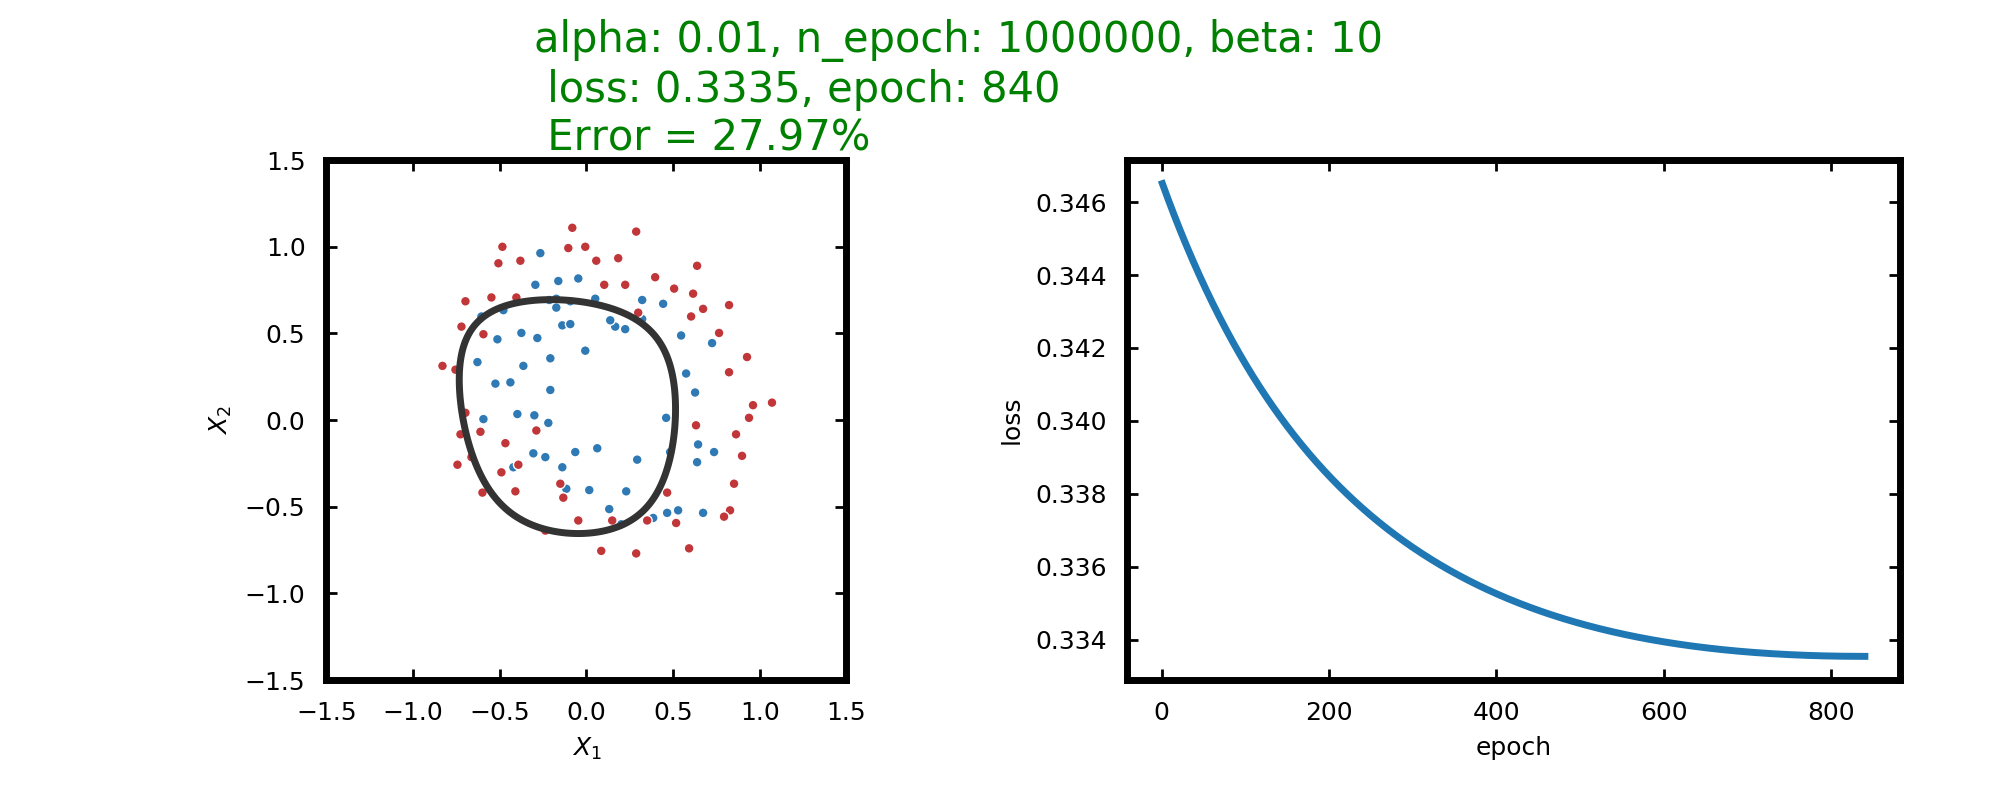
\includegraphics[width=0.85\textwidth]{fig/prob3/alpha_0_01_n_epoch1000000_beta_10.png}
\centering 
\caption{\protect $\beta = 10$}
\label{fig:15th}
\end{figure}

\begin{figure}[H]
\centering
  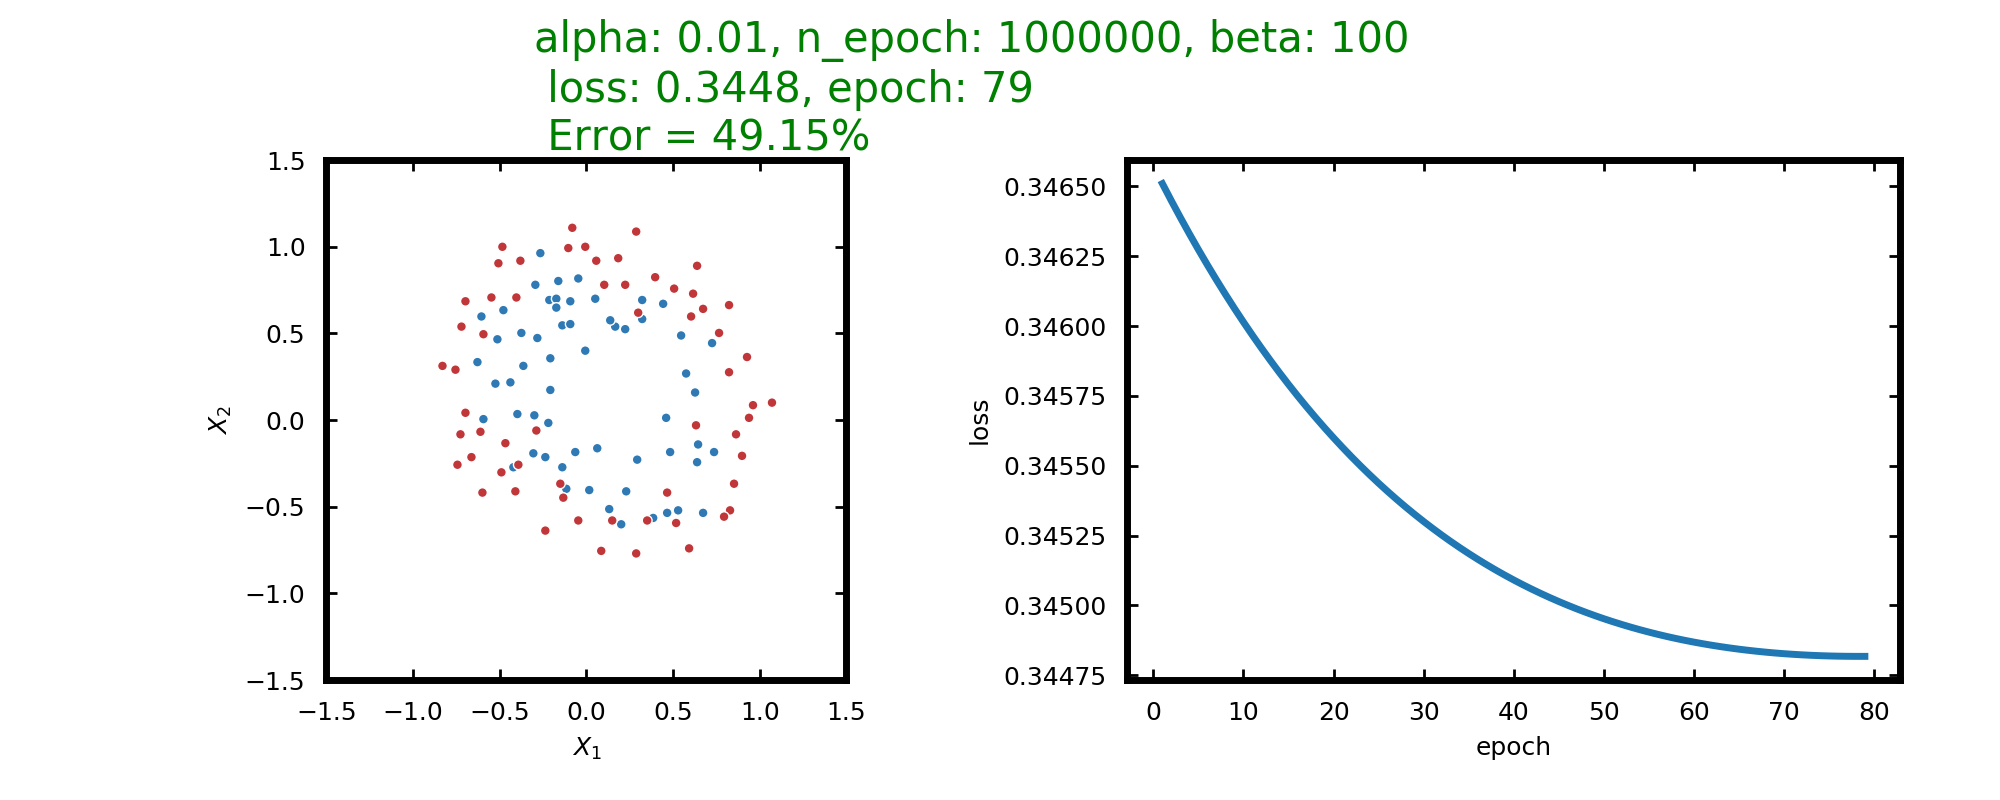
\includegraphics[width=0.85\textwidth]{fig/prob3/alpha_0_01_n_epoch1000000_beta_100.png}
\centering 
\caption{\protect $\beta = 100$}
\label{fig:15th}
\end{figure}



